\Aufgabe[Predicate Abstraction\hfill\textbf{(1.5 Point)}]
Consider the following program:
\begin{verbatim}
void foo(int j, int z) {
  assume(z != 0);
  int i := j;
  while(z != 0) {
      i := i + z;
      if(z > 0)
          z--
      else
          z ++;
  };
  assert(i != j)
}
\end{verbatim}

The {\em assume statement} at the beginning of the function forces the parameter $z$ not to be 0 when the function is called.

\begin{enumerate}

 \item Argue in your own words why the assertion at the end of the program allways holds, i.e., why the error state can never be reached.

 \item Provide a labeled transition system for the given program.

 \item Provide an abstraction for the labeled transition system that uses the predicates $i = j$, $i < j$, $i > j$.

 \item Check whether the error state can be reached in the abstraction, if so state a trace to the error state and refine the abstraction with suitable predicates such that the error state is not reachable anymore.

\end{enumerate}


\textbf{Solution:}\\
\medskip
\begin{enumerate}
\item The call of the method \texttt{\small assume(z != 0)} in the beginning
of the program forces, that the value of the variable $z$ is not $0$. Since
the semantics of \texttt{\small assume(x)}, means that "by assumption \texttt%
{\small x} holds" and by definition an assumption can never being violated.
Thus, the while-loop will be executed at least one time, regardless if the
value of $z$ is positive or negative.

Since the if-condition inside of the loop controls $z$ by decrementing or
incrementing and consequently the variable $i$ will also incremented or
decremented. Thus, the loop will be executed exactly in $|z|$ times. Since  $%
i=j$ is in the precondition of the loop, the loop is guaranteed to terminate
since $z\neq 0$. Hence, after the termination of the while-loop, the case
that $i=j$ will never reached, i.e. it will never hold.
\newpage

\item \textit{Labeled Transiton System (LTS):}

\begin{figure}[th]
\centering
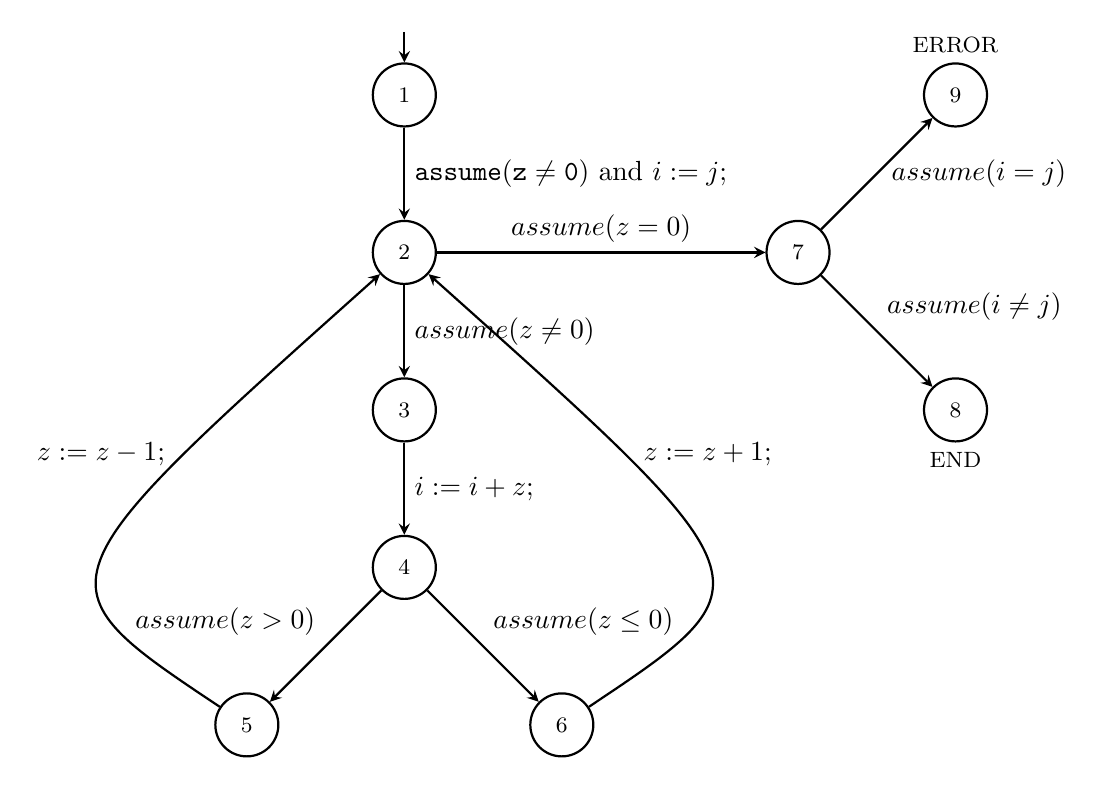
\begin{tikzpicture}[->, >=stealth, line join=bevel]
	\pgfsetlinewidth{1bp}
	\pgfsetcolor{black}

	\tikzstyle{state} = [draw,shape=circle,minimum size=8mm,font=\footnotesize];
	\tikzstyle{accept_state} = [shape=circle, minimum size=8mm, accepting, font=\small, draw];
	\tikzstyle{every path} = [draw, thick];

	\node[state] at (0,10) (1) {$1$};
	\node[state] at (0,8) (2) {$2$}; 
	\node[state] at (0,6) (3) {$3$}; 
	\node[state] at (0,4) (4) {$4$}; 
	\node[state] at (-2,2) (5) {$5$}; 
	\node[state] at (2,2) (6) {$6$}; 
	\node[state] at (5,8) (7) {$7$}; 
	\node[state] at (7,6) (8) [label=below:{\footnotesize END}] {$8$}; 
	\node[state] at (7,10) (9) [label=above:{\footnotesize ERROR}] {$9$}; 

	\draw (0, 10.8) to (1);
	\draw (1) to node[auto] {$\mbox{\fontsize{10}{11}\selectfont $\mathtt{assume(z \neq 0)} \mbox{ and } i := j;$}$} (2);
	\draw (2) to node[auto] {$\mbox{\fontsize{10}{11}\selectfont $assume(z \neq 0)$}$} (3);
	\draw (3) to node[auto] {$\mbox{\fontsize{10}{11}\selectfont $i := i+z;$}$} (4);
	\draw (4) to node[auto, swap] {$\mbox{\fontsize{10}{11}\selectfont $assume(z > 0)$}$} (5);
	\draw (4) to node[auto] {$\mbox{\fontsize{10}{11}\selectfont $assume(z \leq 0)$}$} (6);
	\draw (2) to node[auto] {$\mbox{\fontsize{10}{11}\selectfont $assume(z = 0)$}$} (7);
	\draw (7) to node[auto] {$\mbox{\fontsize{10}{11}\selectfont $assume(i \neq j)$}$} (8);
	\draw (7) to node[right] {$\mbox{\fontsize{10}{11}\selectfont $\,assume(i = j)$}$} (9);
	\draw[->] (5) .. controls (-4.7,3.8) .. (2) node[pos=.75, left] {$z := z-1;\;$};
	\draw[->] (6) .. controls (4.7,3.8) .. (2) node[pos=.75, right] {$\;z := z+1;$};
\end{tikzpicture}
\caption{{\protect\small LTS of the given program.}}
\label{lts_program}
\end{figure}

\item The corresponding predicates for the abstract transition system $%
TS^{abstract}$ (see figure \ref{abstraction_graph}) are defined as follows:%
\begin{equation*}
e\equiv i=j,\quad l\equiv i<j\quad \text{and\quad }g\equiv i>j,
\end{equation*}

where $e$ denotes the case that $(i=j)$ holds and $\overline{e}$ denotes the
that case $(i=j)$ does not hold in the current state. This definition holds
also for the predicates $l$ and $g$.

A possible error trail would be for example $(1,l\overline{g}\overline{e}%
)\rightarrow (2,\overline{l}\overline{g}e)\rightarrow (7,\overline{l}%
\overline{g}e)\rightarrow (9,\overline{l}\overline{g}e)$. Since by the
definition of assumption, an assumption can be never violated, the
error state $(9,\overline{l}\overline{g}e)$ in $TS^{abstract}$ will never
reached.

\begin{figure}[th]
\centering
% Start of code
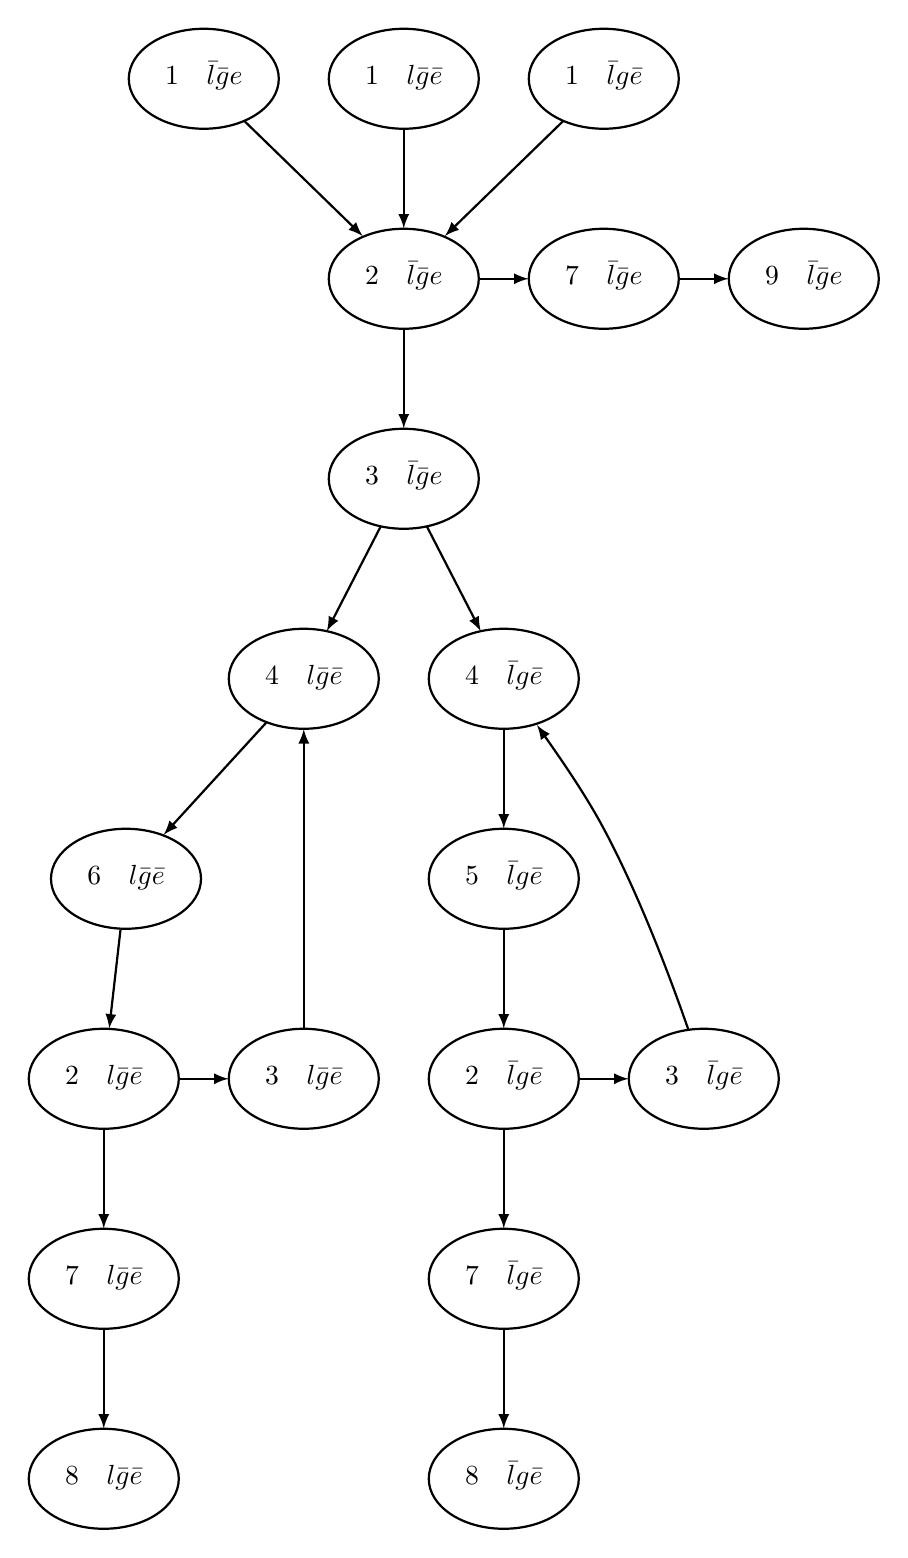
\begin{tikzpicture}[anchor=mid,>=latex,line join=bevel]
%\begin{tikzpicture}[>=latex,line join=bevel]
  \pgfsetlinewidth{1bp}
%%
\pgfsetcolor{black}
  % Edge: 15 -> 17
  \draw [->] (171bp,71.697bp) .. controls (171bp,63.983bp) and (171bp,54.712bp)  .. (171bp,36.104bp);
  % Edge: 5 -> 6
  \draw [->] (126.65bp,360.76bp) .. controls (122.29bp,352.28bp) and (116.85bp,341.71bp)  .. (107.3bp,323.15bp);
  % Edge: 10 -> 12
  \draw [->] (54bp,162bp) .. controls (56.615bp,162bp) and (59.229bp,162bp)  .. (71.93bp,162bp);
  % Edge: 5 -> 7
  \draw [->] (143.35bp,360.76bp) .. controls (147.71bp,352.28bp) and (153.15bp,341.71bp)  .. (162.7bp,323.15bp);
  % Edge: 4 -> 18
  \draw [->] (162bp,450bp) .. controls (164.61bp,450bp) and (167.23bp,450bp)  .. (179.93bp,450bp);
  % Edge: 12 -> 6
  \draw [->] (99bp,180.19bp) .. controls (99bp,204.42bp) and (99bp,248.89bp)  .. (99bp,287.87bp);
  % Edge: 18 -> 19
  \draw [->] (234bp,450bp) .. controls (236.61bp,450bp) and (239.23bp,450bp)  .. (251.93bp,450bp);
  % Edge: 14 -> 16
  \draw [->] (27bp,71.697bp) .. controls (27bp,63.983bp) and (27bp,54.712bp)  .. (27bp,36.104bp);
  % Edge: 4 -> 5
  \draw [->] (135bp,431.7bp) .. controls (135bp,423.98bp) and (135bp,414.71bp)  .. (135bp,396.1bp);
  % Edge: 11 -> 13
  \draw [->] (198bp,162bp) .. controls (200.61bp,162bp) and (203.23bp,162bp)  .. (215.93bp,162bp);
  % Edge: 10 -> 14
  \draw [->] (27bp,143.7bp) .. controls (27bp,135.98bp) and (27bp,126.71bp)  .. (27bp,108.1bp);
  % Edge: 13 -> 7
  \draw [->] (237.38bp,179.88bp) .. controls (231.03bp,198.14bp) and (219.88bp,227.89bp)  .. (207bp,252bp) .. controls (201.73bp,261.86bp) and (195.05bp,272.15bp)  .. (182.95bp,289.32bp);
  % Edge: 1 -> 4
  \draw [->] (77.57bp,506.83bp) .. controls (87.75bp,496.94bp) and (101.52bp,483.55bp)  .. (120.2bp,465.38bp);
  % Edge: 8 -> 10
  \draw [->] (33.022bp,215.7bp) .. controls (32.141bp,207.98bp) and (31.081bp,198.71bp)  .. (28.955bp,180.1bp);
  % Edge: 7 -> 9
  \draw [->] (171bp,287.7bp) .. controls (171bp,279.98bp) and (171bp,270.71bp)  .. (171bp,252.1bp);
  % Edge: 11 -> 15
  \draw [->] (171bp,143.7bp) .. controls (171bp,135.98bp) and (171bp,126.71bp)  .. (171bp,108.1bp);
  % Edge: 3 -> 4
  \draw [->] (192.43bp,506.83bp) .. controls (182.25bp,496.94bp) and (168.48bp,483.55bp)  .. (149.8bp,465.38bp);
  % Edge: 6 -> 8
  \draw [->] (85.427bp,290.15bp) .. controls (76.688bp,280.6bp) and (65.166bp,267.99bp)  .. (48.553bp,249.82bp);
  % Edge: 9 -> 11
  \draw [->] (171bp,215.7bp) .. controls (171bp,207.98bp) and (171bp,198.71bp)  .. (171bp,180.1bp);
  % Edge: 2 -> 4
  \draw [->] (135bp,503.7bp) .. controls (135bp,495.98bp) and (135bp,486.71bp)  .. (135bp,468.1bp);
  % Node: 11
\begin{scope}
  \definecolor{strokecol}{rgb}{0.0,0.0,0.0};
  \pgfsetstrokecolor{strokecol}
  \draw (171bp,162bp) ellipse (27bp and 18bp);
  \draw (171bp,162bp) node {$2 \quad \bar{l}g\bar{e}$};
\end{scope}
  % Node: 10
\begin{scope}
  \definecolor{strokecol}{rgb}{0.0,0.0,0.0};
  \pgfsetstrokecolor{strokecol}
  \draw (27bp,162bp) ellipse (27bp and 18bp);
  \draw (27bp,162bp) node {$2 \quad l\bar{g}\bar{e}$};
\end{scope}
  % Node: 13
\begin{scope}
  \definecolor{strokecol}{rgb}{0.0,0.0,0.0};
  \pgfsetstrokecolor{strokecol}
  \draw (243bp,162bp) ellipse (27bp and 18bp);
  \draw (243bp,162bp) node {$3 \quad \bar{l}g\bar{e}$};
\end{scope}
  % Node: 12
\begin{scope}
  \definecolor{strokecol}{rgb}{0.0,0.0,0.0};
  \pgfsetstrokecolor{strokecol}
  \draw (99bp,162bp) ellipse (27bp and 18bp);
  \draw (99bp,162bp) node {$3 \quad l\bar{g}\bar{e}$};
\end{scope}
  % Node: 15
\begin{scope}
  \definecolor{strokecol}{rgb}{0.0,0.0,0.0};
  \pgfsetstrokecolor{strokecol}
  \draw (171bp,90bp) ellipse (27bp and 18bp);
  \draw (171bp,90bp) node {$7 \quad \bar{l}g\bar{e}$};
\end{scope}
  % Node: 14
\begin{scope}
  \definecolor{strokecol}{rgb}{0.0,0.0,0.0};
  \pgfsetstrokecolor{strokecol}
  \draw (27bp,90bp) ellipse (27bp and 18bp);
  \draw (27bp,90bp) node {$7 \quad l\bar{g}\bar{e}$};
\end{scope}
  % Node: 17
\begin{scope}
  \definecolor{strokecol}{rgb}{0.0,0.0,0.0};
  \pgfsetstrokecolor{strokecol}
  \draw (171bp,18bp) ellipse (27bp and 18bp);
  \draw (171bp,18bp) node {$8 \quad \bar{l}g\bar{e}$};
\end{scope}
  % Node: 16
\begin{scope}
  \definecolor{strokecol}{rgb}{0.0,0.0,0.0};
  \pgfsetstrokecolor{strokecol}
  \draw (27bp,18bp) ellipse (27bp and 18bp);
  \draw (27bp,18bp) node {$8 \quad l\bar{g}\bar{e}$};
\end{scope}
  % Node: 19
\begin{scope}
  \definecolor{strokecol}{rgb}{0.0,0.0,0.0};
  \pgfsetstrokecolor{strokecol}
  \draw (279bp,450bp) ellipse (27bp and 18bp);
  \draw (279bp,450bp) node {$9 \quad \bar{l}\bar{g}e$};
\end{scope}
  % Node: 18
\begin{scope}
  \definecolor{strokecol}{rgb}{0.0,0.0,0.0};
  \pgfsetstrokecolor{strokecol}
  \draw (207bp,450bp) ellipse (27bp and 18bp);
  \draw (207bp,450bp) node {$7 \quad \bar{l}\bar{g}e$};
\end{scope}
  % Node: 1
\begin{scope}
  \definecolor{strokecol}{rgb}{0.0,0.0,0.0};
  \pgfsetstrokecolor{strokecol}
  \draw (63bp,522bp) ellipse (27bp and 18bp);
  \draw (63bp,522bp) node {$1 \quad \bar{l}\bar{g}e$};
\end{scope}
  % Node: 3
\begin{scope}
  \definecolor{strokecol}{rgb}{0.0,0.0,0.0};
  \pgfsetstrokecolor{strokecol}
  \draw (207bp,522bp) ellipse (27bp and 18bp);
  \draw (207bp,522bp) node {$1 \quad \bar{l}g\bar{e}$};
\end{scope}
  % Node: 2
\begin{scope}
  \definecolor{strokecol}{rgb}{0.0,0.0,0.0};
  \pgfsetstrokecolor{strokecol}
  \draw (135bp,522bp) ellipse (27bp and 18bp);
  \draw (135bp,522bp) node {$1 \quad l\bar{g}\bar{e}$};
\end{scope}
  % Node: 5
\begin{scope}
  \definecolor{strokecol}{rgb}{0.0,0.0,0.0};
  \pgfsetstrokecolor{strokecol}
  \draw (135bp,378bp) ellipse (27bp and 18bp);
  \draw (135bp,378bp) node {$3 \quad \bar{l}\bar{g}e$};
\end{scope}
  % Node: 4
\begin{scope}
  \definecolor{strokecol}{rgb}{0.0,0.0,0.0};
  \pgfsetstrokecolor{strokecol}
  \draw (135bp,450bp) ellipse (27bp and 18bp);
  \draw (135bp,450bp) node {$2 \quad \bar{l}\bar{g}e$};
\end{scope}
  % Node: 7
\begin{scope}
  \definecolor{strokecol}{rgb}{0.0,0.0,0.0};
  \pgfsetstrokecolor{strokecol}
  \draw (171bp,306bp) ellipse (27bp and 18bp);
  \draw (171bp,306bp) node {$4 \quad \bar{l}g\bar{e}$};
\end{scope}
  % Node: 6
\begin{scope}
  \definecolor{strokecol}{rgb}{0.0,0.0,0.0};
  \pgfsetstrokecolor{strokecol}
  \draw (99bp,306bp) ellipse (27bp and 18bp);
  \draw (99bp,306bp) node {$4 \quad l\bar{g}\bar{e}$};
\end{scope}
  % Node: 9
\begin{scope}
  \definecolor{strokecol}{rgb}{0.0,0.0,0.0};
  \pgfsetstrokecolor{strokecol}
  \draw (171bp,234bp) ellipse (27bp and 18bp);
  \draw (171bp,234bp) node {$5 \quad \bar{l}g\bar{e}$};
\end{scope}
  % Node: 8
\begin{scope}
  \definecolor{strokecol}{rgb}{0.0,0.0,0.0};
  \pgfsetstrokecolor{strokecol}
  \draw (35bp,234bp) ellipse (27bp and 18bp);
  \draw (35bp,234bp) node {$6 \quad l\bar{g}\bar{e}$};
\end{scope}
%
\end{tikzpicture}
% End of code
\caption{{\protect\small The abstract transition system $TS^{abstract}$ of the above LTS (\ref{lts_program}), where the state $8$ denotes the final \textit{terminal state} and state $9$ the \textit{error state}.}}
\label{abstraction_graph}
\end{figure}

\item By adding a new predicate symbol $z$ to the set of predicates $P=\{l,g,e\}$
of the abstract transition system $TS^{abstract}$, we achieve a new abstract
transition system. The new predicate $z$ denotes the case that $(z\neq 0)$
holds, whereas $\overline{z}$ denotes that $(z\neq 0)$ does not hold in the
current state. Then the resulting abstract transition system is the same as
shown in \textit{c.)}, but without the path to the error state, since the
states $(7,\overline{l}\overline{g}e)$ and $(9,\overline{l}\overline{g}e)$
will never reached.


\end{enumerate}